%\documentclass[10pt]{beamer}
\documentclass[xcolor={dvipsnames}]{beamer}

\usetheme{CambridgeUS}

\definecolor{cambridgedarkorange}{HTML}{9b0014}
\definecolor{cambridgegreen}{RGB}{88,166,24}
\definecolor{cambridgeorange}{HTML}{9b0014}
\definecolor{redUnipd}{HTML}{9b0014}
\definecolor{grayUnipd}{HTML}{444F51}
\definecolor{myblue}{HTML}{317a9b}
%\definecolor{Black}{RGB}{0,62,114}
\newcommand{\bbf}[1]{\textcolor{black}{\bf #1}}
\newcommand{\rbf}[1]{\textcolor{redUnipd}{ #1}}
\usefonttheme{structurebold}
%\usecolortheme[named=myblue]{structure}
\setbeamercolor*{structure}{bg=white,fg=redUnipd}
\setbeamercolor{frametitle}{bg=white,fg=redUnipd}
\setbeamercolor{titlelike}{bg=white,fg=redUnipd}
\setbeamercolor*{palette primary}{use=structure,fg=redUnipd,bg=white}
\setbeamertemplate{navigation symbols}{}
\setbeamertemplate{title page}[default][colsep=-4bp,rounded=true]
%\setbeamercolor*{normal text}{bg=white,fg=black}
%\setbeamertemplate{itemize items}{$\circ$}
%\textopenbullet
%\usepackage{marvosym}
%\setbeamertemplate{itemize items}{$\Neutral$}
\usepackage{booktabs}
\usepackage{pgfpages}
%\pgfpagesuselayout{resize to}[a4paper, 
%                                border shrink=1.5cm,
%                                landscape]
\setbeamertemplate{blocks}[rounded][shadow=false]

\usepackage[T1]{fontenc}
\usepackage{hyperref}
\usepackage[english]{babel}
\usepackage{graphicx}
\usepackage{booktabs}
\usepackage{latexsym}
\usepackage{subfigure}
%\usepackage{enumitem}
\usepackage{amsmath,amssymb}
\usepackage[latin1]{inputenc}
%\setbeamercovered{dynamic}
\usepackage{Sweave}
\usepackage[english]{babel}
\usepackage{tikz,comment,amssymb}
\usetikzlibrary{shapes}
\usepackage{multirow}
\setbeamertemplate{enumerate items}[default]
\setbeamertemplate{section in toc}[sections numbered]
\setbeamertemplate{subsection in toc}[subsections numbered]
\setbeamertemplate{itemize items}[square]
\newcommand{\bb}[1]{\begin{block}{#1}}
\newcommand{\eb}{\end{block}}
\newcommand{\bi}{\begin {itemize}}
\newcommand{\ei}{\end{itemize}}
\newcommand{\be}{\begin {enumerate}}
\newcommand{\ee}{\end{enumerate}}
\linespread{1.05}

\AtBeginSection[] {
  \begin{frame}<beamer>
    \frametitle{Outline}
    \tableofcontents[currentsection]
  \end{frame}
}


\title[]{The Labyrinth of Multiple Testing: How to avoid the pitfall of false positives \\
\vspace*{1cm} \large Introduction to Hypothesis testing}
\subtitle{\vspace*{2cm} \small 12th SISMEC National Congress 2023}
\date{}
\author[\hspace{5cm}]{Livio Finos and Angela Andreella}
% \date{A.A. 2015/2016 }
%\logo{
\includegraphics[scale=.05]{figures/logoUnipd.jpg}}

\begin{document}


\begin{frame}
  \titlepage
\end{frame}

\begin{frame}
    \begin{minipage}[t]{0.45\textwidth}

\includegraphics[width= \textwidth]{Slides/MTP/plaatjes/Finos.jpg}
\begin{itemize}
    \item Full professor in statistics at the University of Padova
    \item \textbf{E-mail}: \\ \href{mailto:livio.finos@unipd.it}{livio.finos@unipd.it} 
\end{itemize}

\end{minipage}\hfill
\begin{minipage}[t]{0.45\textwidth}
  
\includegraphics[width= .95\textwidth]{Slides/MTP/plaatjes/Andreella.jpg}
\begin{itemize}
    \item Researcher in social statistics at the University Ca' Foscari Venezia
    \item \textbf{E-mail}: \href{mailto:angela.andreella@unive.it}{angela.andreella@unive.it} 
\end{itemize}

\end{minipage}
\end{frame}

\section{Introduction}

\begin{frame}
\frametitle{American Statistical Association's\\
Ethical Guidelines for Statistical Practice}

% \begin{tabular}{l|l}
Recognize that any frequentist %& $\mathcal{H}=\{A\}$ \\ 
statistical test has a random %&decision rule: reject $A$ if $p_{A}\leq \alpha$\\ 
chance of indicating \textbf{significance} %&$\Pr(p_A\leq \alpha) \leq \alpha$ when $A$ true \\  
when it is \textbf{not really present}. %& (probability of type I error)\\ 
% &\\
\bigskip

Selecting the one ``significant'' % & $\mathcal{H}=\{A, B, C,D\}$ \\
result from a multiplicity of parallel  %& $p_{\min}=\min(p_A,p_B,p_C,p_D)$ \\
tests poses a grave risk of an  %& $\Pr(p_{\min}\leq \alpha)\leq 4\alpha$ when all true \\
\textbf{incorrect conclusion}.   %& (probability of at least one type I error) \\
% &\\
\bigskip

Failure to disclose the full extent % & \\% \\
of tests and their results in such  %&  \\
a case would be highly misleading. %& \\
% \end{tabular}
\pause

\bigskip
e.g. VaxGen's AIDSVAX trial \ldots
\end{frame}

%%%%%%%%%%%%%%%%%%%%%%%%%%%%%%%%%%%%%%%%%%%%%%%%%%%%%%%%%%%%%%%%%%%%%%%%%%%%%%%%%%%%%%%%%%%%%%%%%%%%%%
\begin{frame}
\frametitle{VaxGen's AIDSVAX trial}


VaxGen announced the results of the \textbf{first-ever efficacy trial} of an AIDS vaccine on 24 February 2003:

\bigskip

%the vaccine failed to prevent HIV infection (primary endpoint):

\begin{center}
\textbf{The vaccine prevent HIV infection?}
\end{center}

\bigskip


\begin{tikzpicture}
\node at (0,0.25) {\small{All subjects}};
\node at (2,1) {\small{Total}};
\node at (3.2,1) {\small{Infected}};
\draw (-.8,0.8) -- (3.8,0.8);
\node[text=cambridgegreen]  at (2,0.5) {\small{1679}};
\node[text=cambridgegreen]  at (3.2,0.5) {\small{96}};
\node[text=cambridgeorange]  at (2,0) {\small{3330}};
\node[text=cambridgeorange]  at (3.2,0) {\small{191}};
\draw (-.8,-0.3) -- (3.8,-0.3);
\draw[fill=cambridgegreen] (4,0.3) rectangle +(1.16,0.4);
\draw[fill=cambridgeorange] (4,-0.2) rectangle +(1.14,0.4);
\node[text=cambridgegreen]  at (5.7,0.5) {\small{5.8\%}};
\node[text=cambridgeorange]  at (5.7,0) {\small{5.7\%}};
\node[text=cambridgegreen]  at (8,0.5) {\small{PLACEBO}};
\node[text=cambridgeorange]  at (8,0) {\small{VACCINE}};
\end{tikzpicture}


\bigskip


\emph{"We saw absolutely no difference between the vaccine and placebo groups. Everyone was pretty depressed."}

\bigskip

but the next day...

\end{frame}
%%%%%%%%%%%%%%%%%%%%%%%%%%%%%%%%%%%%%%%%%%%%%%%%%%%%%%%%%%%%%%%%%%%%%%%%%%%%%%%%%%%%%%%%%%%%%%%%%%%%%%
\begin{frame}
\frametitle{VaxGen's AIDSVAX trial}

...by \textbf{broking the data down into racial groups} -- which they say was part of the original design -- the vaccine appeared to have worked in blacks:

%they broke the data down into racial groups, the vaccine appeared to have worked in blacks:

\bigskip

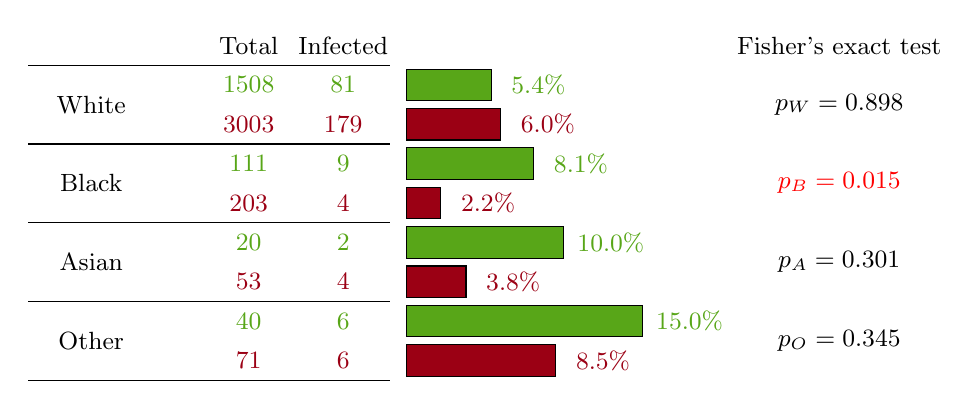
\begin{tikzpicture}
\node  at (9.5,0.25) {\small{$p_W = 0.898$}};
\node[text=red]  at (9.5,-0.75) {\small{$p_B = 0.015$}};
\node  at (9.5,-1.75) {\small{$p_A = 0.301$}};
\node  at (9.5,-2.75) {\small{$p_O = 0.345$}};

\node at (9.5,1) {\small{Fisher's exact test}};
\node at (0,0.25) {\small{White}};
\node at (2,1) {\small{Total}};
\node at (3.2,1) {\small{Infected}};
\draw (-.8,0.75) -- (3.8,0.75);
\node[text=cambridgegreen]  at (2,0.5) {\small{1508}};
\node[text=cambridgegreen]  at (3.2,0.5) {\small{81}};
\node[text=cambridgeorange]  at (2,0) {\small{3003}};
\node[text=cambridgeorange]  at (3.2,0) {\small{179}};
\draw (-.8,-0.25) -- (3.8,-0.25);
\node[text=cambridgegreen]  at (2,-0.5) {\small{111}};
\node[text=cambridgegreen]  at (3.2,-0.5) {\small{9}};
\node[text=cambridgeorange]  at (2,-1) {\small{203}};
\node[text=cambridgeorange]  at (3.2,-1) {\small{4}};
\draw (-.8,-1.25) -- (3.8,-1.25);
\node[text=cambridgegreen]  at (2,-1.5) {\small{20}};
\node[text=cambridgegreen]  at (3.2,-1.5) {\small{2}};
\node[text=cambridgeorange]  at (2,-2) {\small{53}};
\node[text=cambridgeorange]  at (3.2,-2) {\small{4}};
\draw (-.8,-2.25) -- (3.8,-2.25);
\node[text=cambridgegreen]  at (2,-2.5) {\small{40}};
\node[text=cambridgegreen]  at (3.2,-2.5) {\small{6}};
\node[text=cambridgeorange]  at (2,-3) {\small{71}};
\node[text=cambridgeorange]  at (3.2,-3) {\small{6}};
\draw (-.8,-3.25) -- (3.8,-3.25);
\node at (0,-.75) {\small{Black}};
\node at (0,-1.75) {\small{Asian}};
\node at (0,-2.75) {\small{Other}};
\draw[fill=cambridgegreen] (4,0.3) rectangle +(1.08,0.4);
\draw[fill=cambridgeorange] (4,-0.2) rectangle +(1.2,0.4);
\node[text=cambridgegreen]  at (5.68,0.5) {\small{5.4\%}};
\node[text=cambridgeorange]  at (5.8,0) {\small{6.0\%}};
\draw[fill=cambridgegreen] (4,-0.7) rectangle +(1.62,0.4);
\draw[fill=cambridgeorange] (4,-1.2) rectangle +(0.44,0.4);
\node[text=cambridgegreen]  at (6.22,-.5) {\small{8.1\%}};
\node[text=cambridgeorange]  at (5.04,-1) {\small{2.2\%}};
\draw[fill=cambridgegreen] (4,-1.7) rectangle +(2,0.4);
\draw[fill=cambridgeorange] (4,-2.2) rectangle +(0.76,0.4);
\node[text=cambridgegreen]  at (6.6,-1.5) {\small{10.0\%}};
\node[text=cambridgeorange]  at (5.36,-2) {\small{3.8\%}};
\draw[fill=cambridgegreen] (4,-2.7) rectangle +(3,0.4);
\draw[fill=cambridgeorange] (4,-3.2) rectangle +(1.9,0.4);
\node[text=cambridgegreen]  at (7.6,-2.5) {\small{15.0\%}};
\node[text=cambridgeorange]  at (6.5,-3) {\small{8.5\%}};
\end{tikzpicture}

\vspace{.1cm}

\emph{"The numbers were small, which concerned us, but the result was highly statistically significant. They were pretty incredible results."}

\end{frame}
%%%%%%%%%%%%%%%%%%%%%%%%%%%%%%%%%%%%%%%%%%%%%%%%%%%%%%%%%%%%%%%%%%%%%%%%%%%%%%%%%%%%%%%%%%%%%%%%%%%%%%

\begin{frame}
\frametitle{Criticisms}

\begin{enumerate}
\item \textcolor{cambridgedarkorange}{\textbf{Failure to account for multiplicity}}

\bigskip 

\emph{"The p-values were not adjusted.''}
% 
% \bigskip
% 
% \textcolor{cambridgedarkorange}{Decision rule:} reject $H\in \mathcal{H}$ if $p_H\leq \alpha^{\mathrm{adj}}$\\
% \textcolor{cambridgedarkorange}{Familywise Error:} $\mathrm{FWE}=\Pr(\mathrm{at\,\,least\,\,one\,\,type\,\,I\,\,error})$
% 
% \begin{eqnarray*}
% \mathrm{FWE} =  1-(1-\alpha^{\mathrm{adj}})^{4} = 
% \left\{  \begin{array}{ll}
%     0.187 & \mathrm{if\,\,} \alpha^{\mathrm{adj}}=0.05\\ 
%     0.05 & \mathrm{if\,\,} \alpha^{\mathrm{adj}}=0.0127\\ 
%   \end{array}\right.
% \end{eqnarray*}
% when all null hypotheses are true


\bigskip 

\item \textcolor{cambridgedarkorange}{\textbf{Selective reporting (data snooping)}}

\bigskip 

\emph{"It's all murky because it's all post hoc analysis. They might as well do a subgroup analysis based on signs of the zodiac."}

\bigskip

\textbf{If you torture your data long enough, they will confess to you whatever you want to hear!}
\end{enumerate}

\end{frame}
%%%%%%%%%%%%%%%%%%%%%%%%%%%%%%%%%%%%%%%%%%%%%%%%%%%%%%%%%%%%%%%%%%%%%%%%%%%%%%%%%%%%%%%%%%%%%%%%%%%%%%
\begin{frame}
\frametitle{Revived interest in multiple testing}

\large{``-omics''}   \\
\scriptsize{e.g., genomics experiments with microarray data: which genes are differentially expressed?}

\large{model selection}\\
\scriptsize{e.g., multiple regression: which coefficients matter?}

\large{...}


\textbf{\rbf{Clinical trials}}
\begin{columns}[t]
\column{0.45\textwidth}
\textcolor{cambridgedarkorange}{sources of multiplicity}
\begin{itemize}
\item multiple endpoints
\item several treatments
\item multiple time points
\item subgroup analysis
\item interim analysis
\item $\ldots$
\end{itemize}

\column{0.45\textwidth}
\textcolor{cambridgedarkorange}{regulatory guidelines}
\begin{itemize}
\item statistical principles for clinical trials (ICH E9)
\item points
to consider on multiplicity issues in clinical
trials (EMEA)
\item $\ldots$
\end{itemize}
\end{columns}




\end{frame}

\section{Hypothesis testing}

\subsection{Individual hypothesis testing}
\begin{frame}
\frametitle{Hypothesis Testing: One Single Test}

\rbf{Two Hypotheses under comparison}

\begin{itemize}
\item $H_0$: two groups are \textbf{Equal}, no relationship between $X$ and $Y$. 
\item $H_1$: two groups are \textbf{Different}, there is a relationship between $X$ and $Y$.
\end{itemize}

\bigskip

Each test produces a p-value $p$: \\  
\vspace{.5cm}
if $\boxed{p\leq .05}$ ($\alpha=.05$), we \textbf{reject} $H_0$ (and lean towards $H_1$).
\end{frame}

\begin{frame}
\frametitle{Errors}

\begin{table}[]
\centering
\begin{tabular}{@{}ll|ll@{}}
&              & \multicolumn{2}{c}{\textbf{Null hypothesis}}     \\ & \textbf{}    & \multicolumn{1}{c}{\begin{tabular}[c]{@{}c@{}}False\\ (two groups are different)\end{tabular}} & \multicolumn{1}{c}{\begin{tabular}[c]{@{}c@{}}True\\ (two group are equal)\end{tabular}} \\ \midrule
\multicolumn{1}{c}{}                       & Rejected     & \multicolumn{1}{l|}{{\color[HTML]{3166FF} True discovery}}                                     & {\color[HTML]{9A0000} Type I error}                                                      \\
\multicolumn{1}{c}{\multirow{-2}{*}{\textbf{Test}}} & Not rejected & \multicolumn{1}{l|}{{\color[HTML]{9A0000} Type II error}}                                      & {\color[HTML]{3531FF} True negative}                                                    
\end{tabular}
\end{table}

\bigskip

\begin{itemize}
\item \textbf{Type I} (false positive): \textbf{Reject} $H_0$ when it is \textbf{True} \\
$\mathbb{P}(\text{\rbf{Type I Error}})=\mathbb{P}(p\leq .05 | H_0)=.05$
\vspace{.2cm}
\item \textbf{Type II} (false negative): \textbf{Fail} to reject $H_0$ when it is \textbf{False} \\
$\mathbb{P}(\text{\rbf{Type II Error}})=\mathbb{P}(p> .05 | H_1)$\\
\vspace{.2cm}
\bbf{Power}:  $\mathbb{P}(p\leq .05 | H_1) =  1-\mathbb{P}(p>.05 | H_1) = 1-\mathbb{P}(\text{\rbf{Type II Error}})$
\end{itemize}
\end{frame}

\begin{frame}
\frametitle{Asymmetric Importance of Errors}

\begin{center}
Control $\mathbb{P}(\text{\rbf{Type I Error}})$ (e.g., $\leq 0.05$) \\

    and \\

find the test with the maximum \textbf{Power} (minimum $\text{\rbf{Type II Error}}$)
\end{center}

\bigskip

\textit{It's important to remember that:}
\begin{itemize}
\item[-] \textbf{A significant p-value} ($p\leq\alpha$) allows us to think that $H_1$ is true, while
\item[-] \textbf{A non-significant p-value} ($p>\alpha$) does NOT allow us to think that $H_0$ is true; we simply don't have enough evidence to reject it.
\end{itemize}
\end{frame}

\begin{frame}
\frametitle{Type I Error}

%$\mathbb{P}(p\leq .05 | H_0:\textrm{two groups are \textbf{Equal}})=?$\\
Suppose $H_0: \mu_1-\mu_2=0$ and $H_1: \mu_1-\mu_2<0$\\
test statistic $T=\frac{\bar{x}_1-\bar{x}_2}{\hat{\sigma}}$ ( $\hat{\sigma}$ estimate of the std dev of $\bar{x}_1-\bar{x}_2$)\\
under $H_0$: $T\sim t_{n_1+n_2-2}$, then
\begin{eqnarray*}
\mathbb{P}(T\leq t_\alpha | H_0) =\alpha \ \forall \alpha\\
\mathbb{P}(F(T)\leq F(t_\alpha) | H_0) =\alpha \ \forall \alpha\\
\mathbb{P}(P \leq \alpha | H_0) =\alpha \ \forall \alpha
\end{eqnarray*}
\vspace{-1.2cm}

\begin{minipage}{0.45\textwidth}
\centering
consequently, $P\sim U(0,1)$
\end{minipage}\hfill
\begin{minipage}{0.55\textwidth}
 \hspace{1cm} 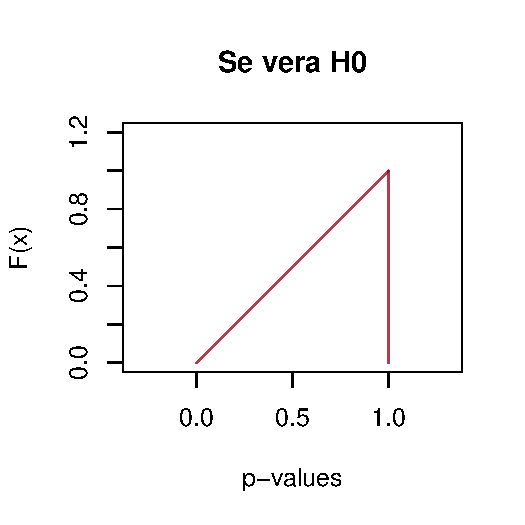
\includegraphics[width= .85\textwidth]{Slides/MTP/plaatjes/cdf_uniform}
\end{minipage}

\end{frame}

\begin{frame}
\frametitle{Type I Error}

\begin{overprint}
\only<1> {Under $H_0$, the p-value is a \rbf{uniform random variable} $U(0,1)$}
\only<2> {\rbf{Type I Error}: $\mathbb{P}(p\leq .05 |H_0)=.05$} % (or at least $\leq .05$)}
\end{overprint} 
\begin{overprint} 
\onslide<1> \centerline{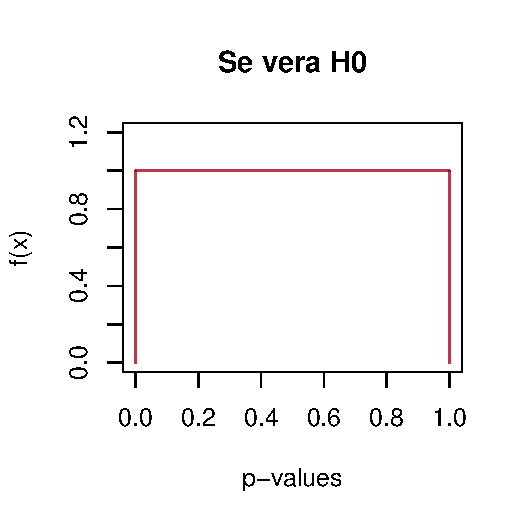
\includegraphics[width=7.5cm]{plaatjes/uniform1}}
\onslide<2> \centerline{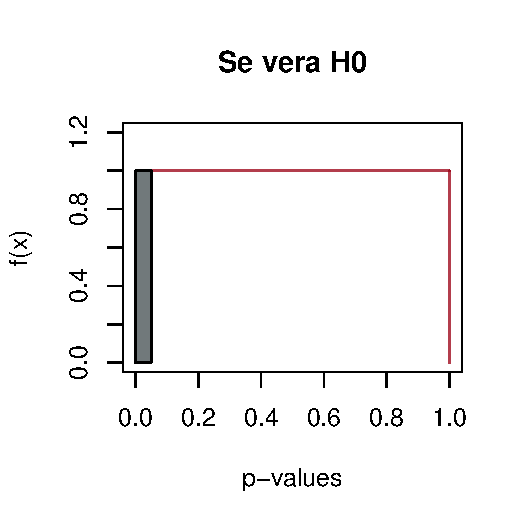
\includegraphics[width=7.5cm]{plaatjes/uniform2}}
\end{overprint} 
\end{frame}

\begin{frame}
\frametitle{Power}

%$\mathbb{P}(p\leq .05 | H_1: \textrm{two groups are \textbf{Different}})$

\begin{overprint}
\only<1> {Under $H_1$, the p-value is \rbf{stochastically smaller} than a uniform random variable $U(0,1)$ (No test distortion)}
\only<2> {Under $H_1$: $\mathbb{P}(p\leq .05 |H_1)>.05$, in our case $= .74$\\ }
\end{overprint}
\begin{overprint} 
\onslide<1> \centerline{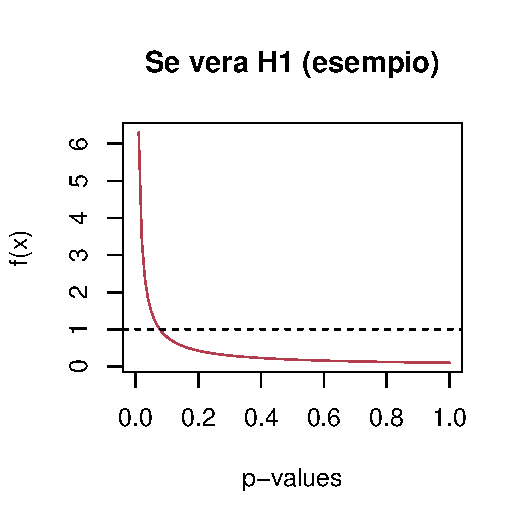
\includegraphics[width=7.5cm]{plaatjes/beta1}}
\onslide<2> \centerline{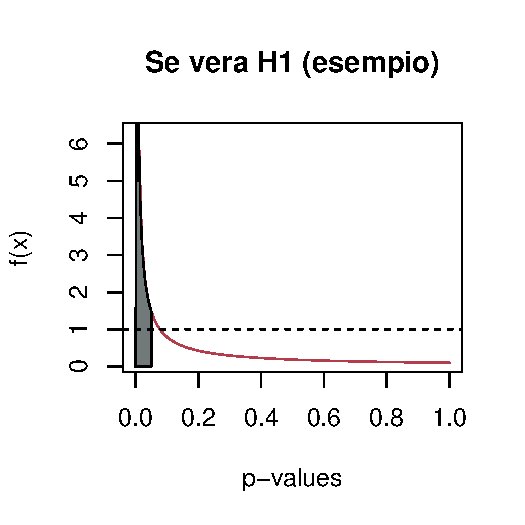
\includegraphics[width=7.5cm]{plaatjes/beta2}}
\end{overprint} 
\end{frame}

\subsection{Multiple hypothesis testing}

\begin{frame}
\frametitle{Hypothesis testing: Multiple Tests}

The goal is to test $m \ge 2$ hypotheses simultaneously from the same data.

\bigskip

Each test carries the risk of making a \rbf{Type I error} $\rightarrow$ the risk of having \textbf{ AT LEAST one} may become unmanageable.    
\end{frame}


\begin{frame}
\frametitle{Two Tests (Independent) Case}

\textbf{\rbf{ESEMPIO}}

\bigskip

Probability of \textbf{ AT LEAST one} (false) rejection?\
\bigskip
\begin{align*}
\mathbb{P}(p_1\leq .05 \cup p_2\leq .05 | H_0) &= 
.05+.05-(.05\cdot .05)=1-(1-.05)^2 \\
&=.0975=1-(1-\alpha)^2 > \alpha
\end{align*}

%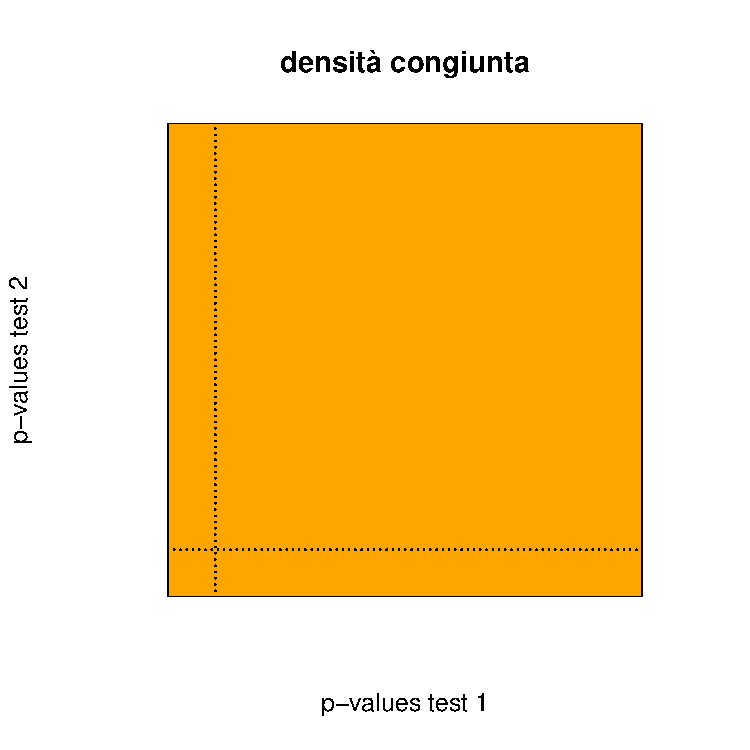
\includegraphics[scale=.5]{plaatjes/bivaH0indep}

\end{frame}

\begin{frame}{Multiple Tests}
    \begin{figure}
        \centering
        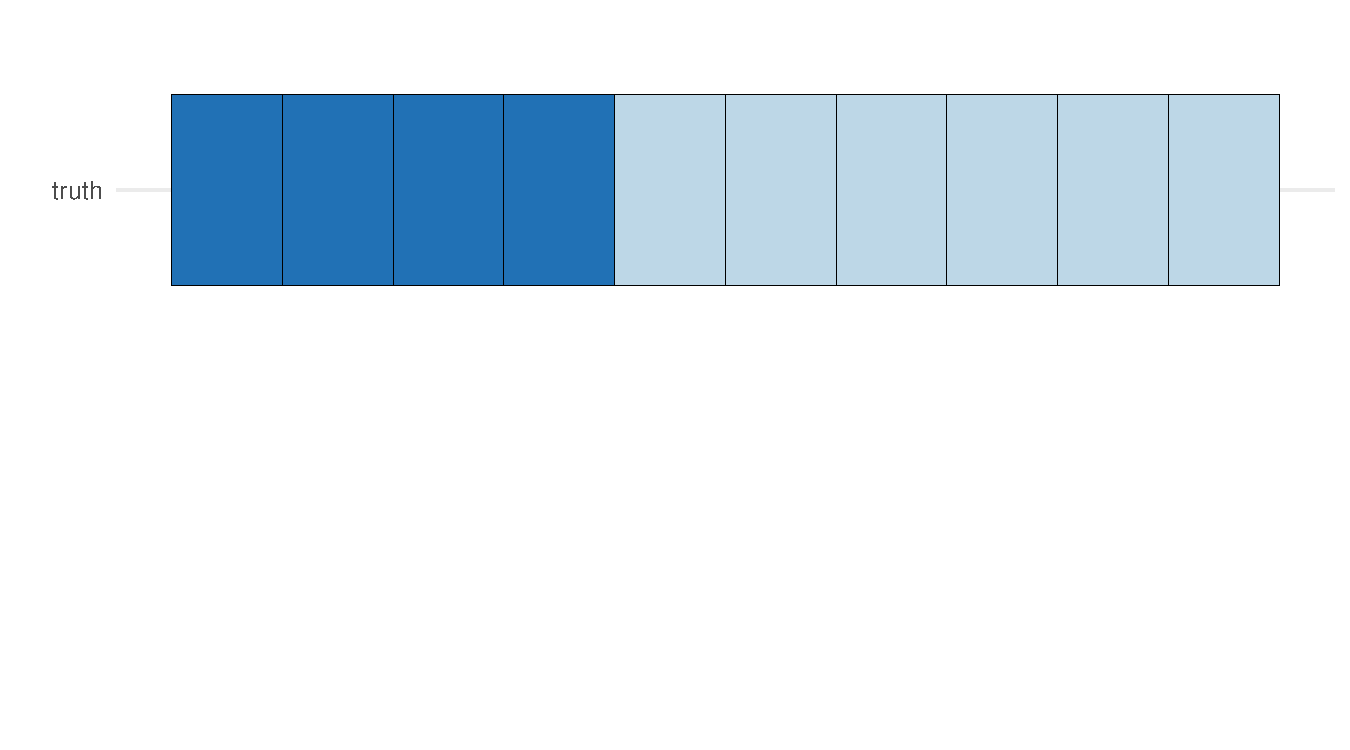
\includegraphics[width = \textwidth]{Slides/MTP/plaatjes/mt1.pdf}

    \end{figure}
\end{frame}

\begin{frame}{Multiple Tests}
    \begin{figure}
        \centering
        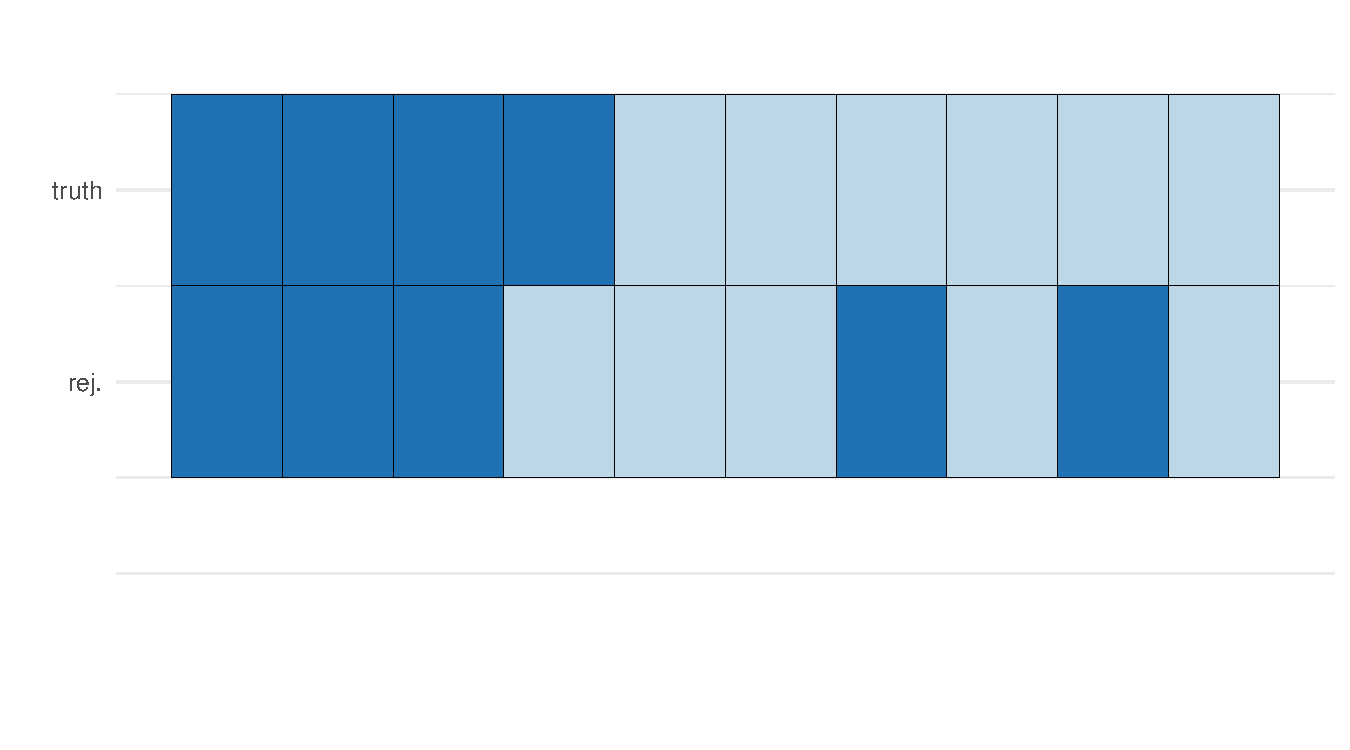
\includegraphics[width = \textwidth]{Slides/MTP/plaatjes/mt2.pdf}
    \end{figure}
\end{frame}

\begin{frame}{Multiple Tests}
    \begin{figure}
        \centering
        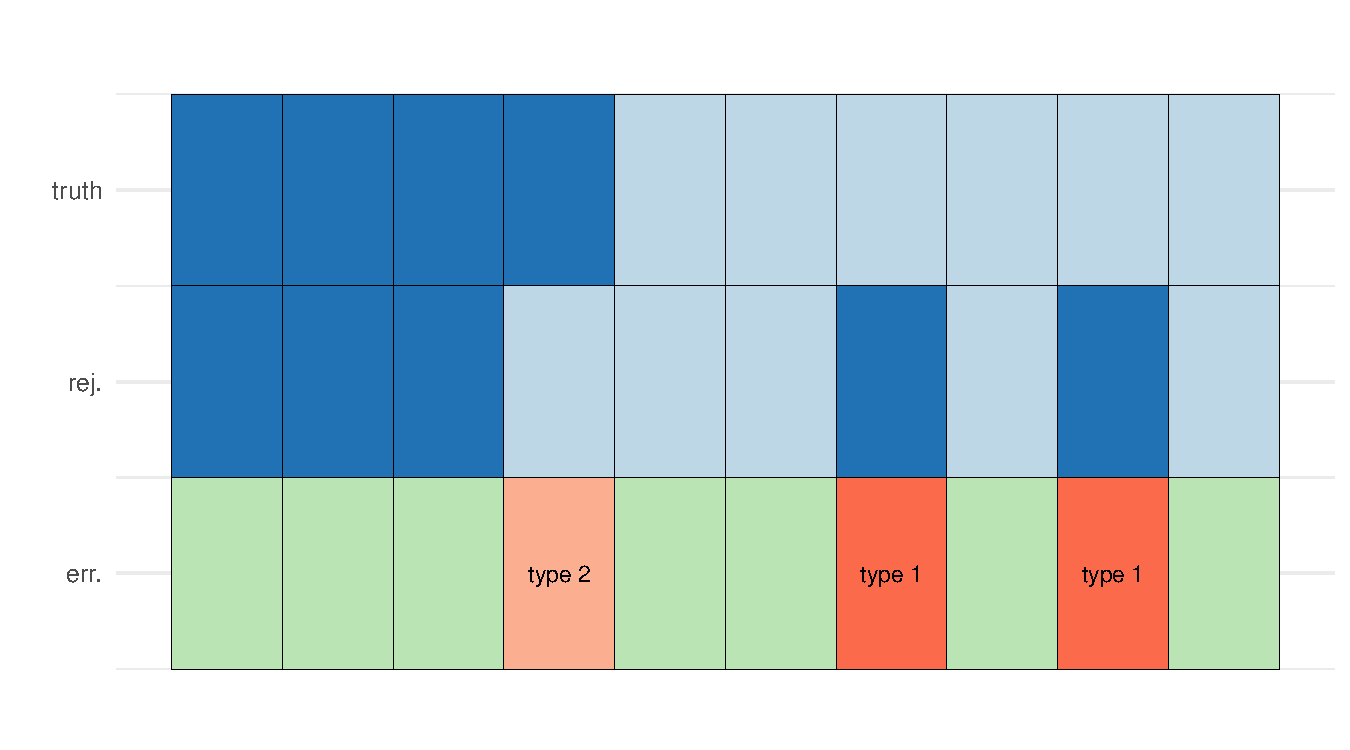
\includegraphics[width = \textwidth]{Slides/MTP/plaatjes/mt3.pdf}

    \end{figure}

\end{frame}

\begin{frame}{Error control}

\begin{table}[]
\centering
\begin{tabular}{@{}ll|ll@{}|l}
&              & \multicolumn{2}{c|}{\textbf{Null hypothesis}}  &   \\ 
& \textbf{}    & \multicolumn{1}{c}{\begin{tabular}[c]{@{}c@{}}False\end{tabular}} & \multicolumn{1}{c}{\begin{tabular}[c]{@{}c@{}}True\end{tabular}} &  \multicolumn{1}{|l}{Tot}\\ 
\midrule
\multicolumn{1}{c}{}                       & Rejected     & \multicolumn{1}{l}{{\color[HTML]{3166FF} $S$}}                                     & {\color[HTML]{9A0000} $V$ (false discoveries)}  &  {\color[HTML]{16c155} $R$}  \\
\multicolumn{1}{c}{\multirow{-2}{*}{\tetxbf{Test}}} & Not rejected & \multicolumn{1}{l}{{\color[HTML]{9A0000} $T$}}                                      & {\color[HTML]{3531FF} $U$}     &   $m - {\color[HTML]{16c155} R} $  \\    \midrule
\multicolumn{1}{c}{}                       & Tot     & \multicolumn{1}{l}{$m_1$}                                     & $m_0$  &  $m$ \\
\end{tabular}
\end{table}
\bigskip

\rbf{Probability of AT LEAST one false rejection:} \\
\begin{equation*}
\mathbb{P}(\textcolor{redUnipd}{V} >0) = 1- (1-\alpha)^m
\end{equation*}

\bigskip

This quickly becomes a problem if $m$ becomes large ...
\end{frame}


%\begin{frame}
%\frametitle{Tests on multiple features}

%\bb{$m$ independent p-values}
%If we reject the hypothesis when $p\leq \alpha$
%\eb
%\bb{Probability of AT LEAST one false rejection:}
%$P = 1- (1-\alpha)^m$
%\eb

%\pause
%\bigskip
%This quickly becomes a problem if $m$ becomes large ...

%\end{frame}

\begin{frame}
\frametitle{Error control}
\begin{figure}
    \centering
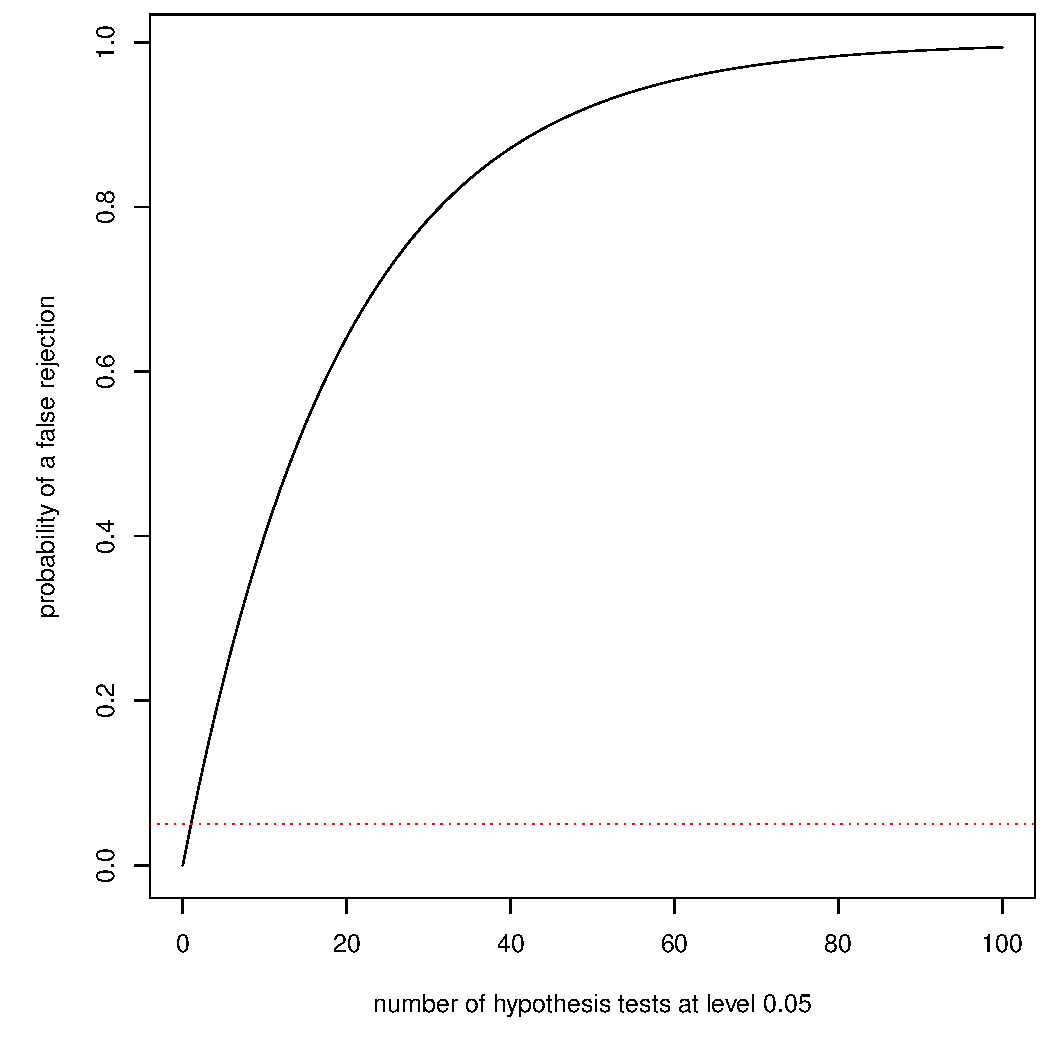
\includegraphics[width = .6\textwidth]{plaatjes/typeI}
\end{figure}
\end{frame}


\begin{frame}
\frametitle{Type I error}
\begin{itemize}
    \item How to \textbf{define} the \rbf{Type I error} when there are many hypotheses?
    \bigskip
    \item Which procedures \textbf{control} this error?
\end{itemize}
\end{frame}

\end{document}


